\chapter{Introduction}
We, as a society nowadays, are in constant demand for energy. Although,
even with the development of calculating, conducting and studying it, we
don't really know what the energy is, we are depending on that abstract
quantity. One might probably say that to study physics is to endure to
study energy in its every possible form. There's a brilliant quote from
Bill Bryson that: ``Energy is liberated matter, matter is energy waiting
to happen.'' What might be incredible is that from this strictly
mathematical quantity we can deduct anything. And what's also important
it is as arbitrary as it gets, depending only on one's reference. From
energy we can create few more important quantities such as \emph{power}
P, which is simply the energy provided per unit time, so:

$$E = \int P\left( t \right)dt$$

The energy will be represented in J (Joules) or eV (electron
volt), which directly describes energy of elementary charge body
(\(e \approx 1.602*10^{- 19}C)\) in 1V (Volt) potential.

$$1eV = 1.602*10^{- 19}J$$

Power will be then represented in W (Watts) (\(W = \frac{J}{s}\ ).\)

The rise of energy consumption has proven that in the future we will
almost certainly require even more. From Global Energy Perspective paper 
\cite{Insights2019} we can learn that:

\begin{itemize}
\item
  Global energy demand will reach plateau at around 2035 despite strong
  population expansion and economic growth thanks to emphasis on
  renewable sources, more efficient service industries or more efficient
  industrial regions

\item
  The energy demand and economic growth became ``decoupled'' for the
  first time in history

\item
  Renewables will provide more than half the electricity after 2035

\end{itemize}

The reader is strongly recommended to take a look at the document.

With saying that we can produce energy there's a slick trick given with
the phrase. Energy cannot be simply created, it is just converted from
another source so nothing is ever lost or miraculously made. The
problems we need to struggle with are then being able to obtain as much
energy from the energy source as it is possible and of course, as
humankind society is governed by money, keep the cost lowest. There is
plenty of different energy sources that we learned to receive energy
from. In Figure \ref{fig:ensour} we can see the most vivid ones nowadays. But with
the human demand fulfilment come great damages and soon depleting
resources of many energy sources such as fossil fuels.

\begin{figure}[h]
\centering
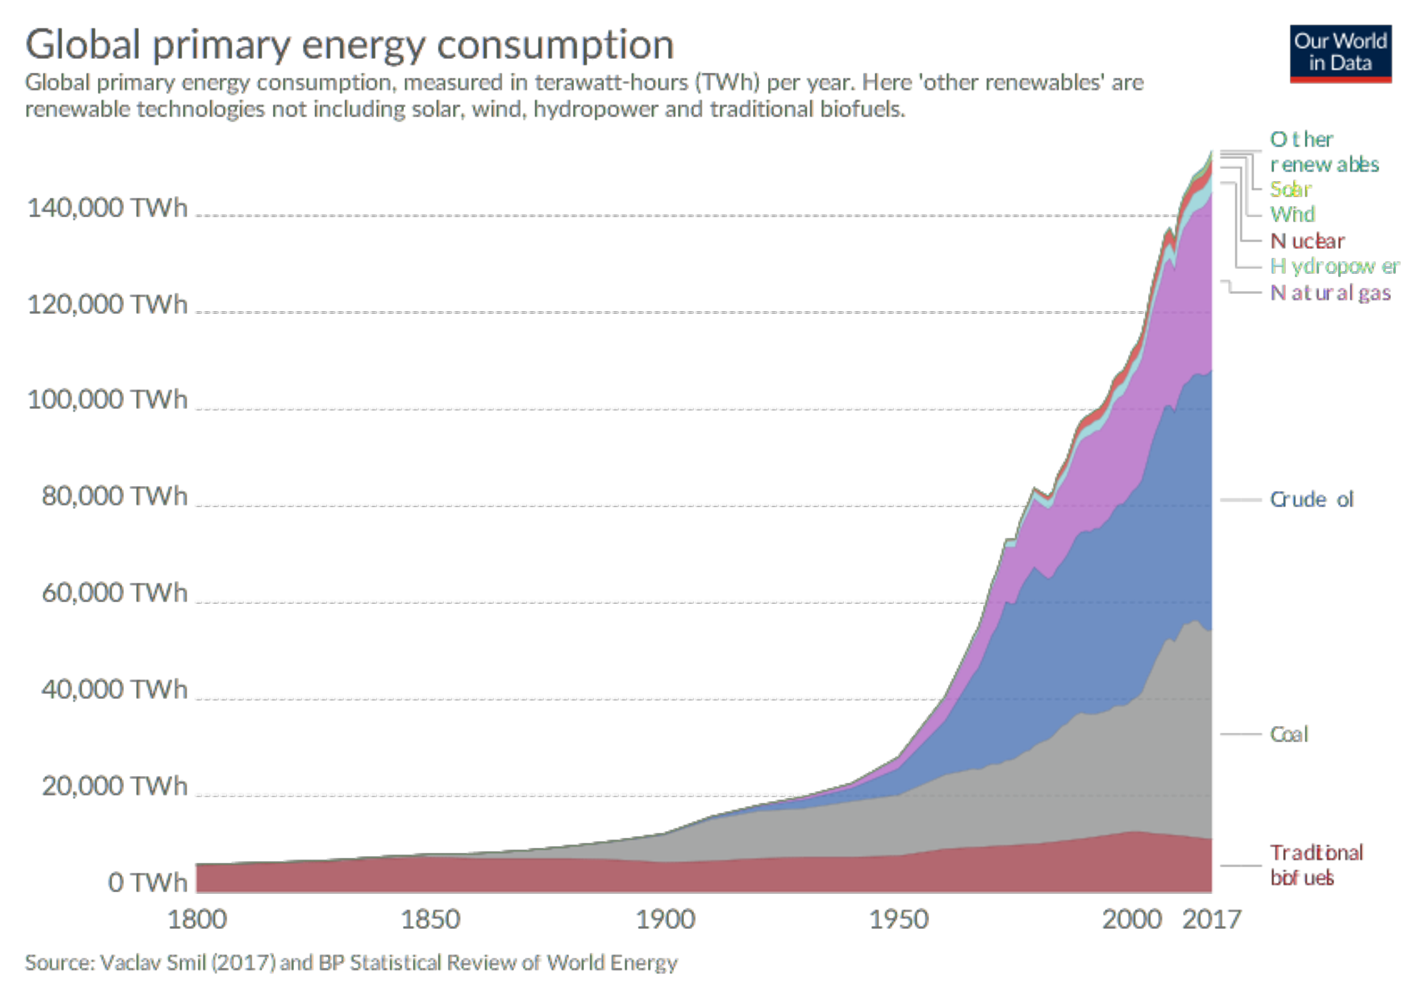
\includegraphics[width=\textwidth]{global-primary-energy}
\caption{Energy sources contribution in world scale
\cite{2019}}
\label{fig:ensour}
\end{figure}

The necessity of searching new possible ways to harness it through renewable sources has become a global issue. Our concern of the environment had never been that serious before. Not only the change of methods for energy production must be enhanced because of this demand but we need to be strictly aware of the World's urging trepidation of Global Warming of which evidence is provided for example here \cite{Nasa2019}.

\newpage

Among all of the ideas created in a past few decades, solar energy is
believed by many to be the most reliable and promising. It can be
directly converted into electricity, heat or chemical energy and our
only star seems to be an infinite power resource for us. In the last ten
years the world solar PV electricity production has grown impressively,
being almost three times bigger in 2016, than in 2010 \cite{2018}. In theory,
the Sun has the potential to fulfil earth's energy demand if it is not
for the technology. Annually, nearly 10\textsuperscript{18} EJ of energy
reaches our planet and of that 10\textsuperscript{4} EJ is claimed to be
harvestable. The possibility of converting the solar energy into
electric energy has been studied since discovery of the basic
photovoltaic effect and the development of semiconductor technologies.

\begin{figure}[h]
\label{fig:annual} 
\centering
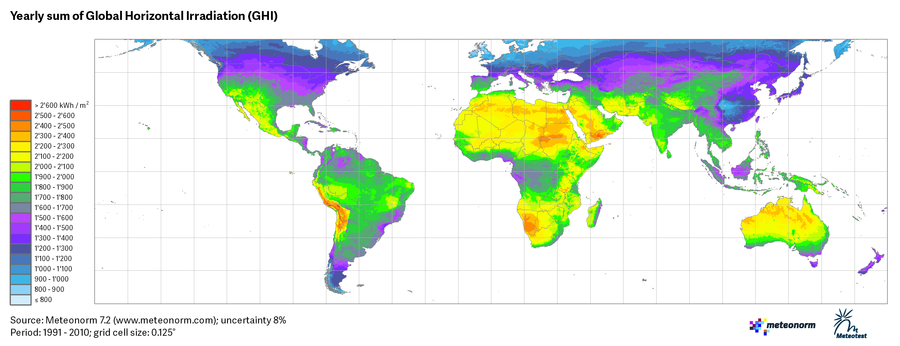
\includegraphics[width=\textwidth]{annual}
\caption{Annual yearly sum of Global Horizontal Irradiation
\cite{1991-2010}}
\end{figure}